%\chapter*{} \label{chapitre6-discussion} % "*" pour ne pas afficher le nom de chapitre
\setcounter{section}{0} % 
%\renewcommand*{\theHsection}{chY.\the\value{section}} % version pour la partie méthodes
% See https://tex.stackexchange.com/questions/71162/reset-section-numbering-between-unnumbered-chapters
\renewcommand*{\theHsection}{\theHchapter.\the\value{section}} % différent de l'intro et méthodes, allez savoir pourquoi !

% COVER PAGE
\centerline{\bfseries\textcolor{bleusection}{ \Huge Discussion générale}}  

\bigskip

% Figure cover
\begin{figure}[H] 
	\begin{center}
	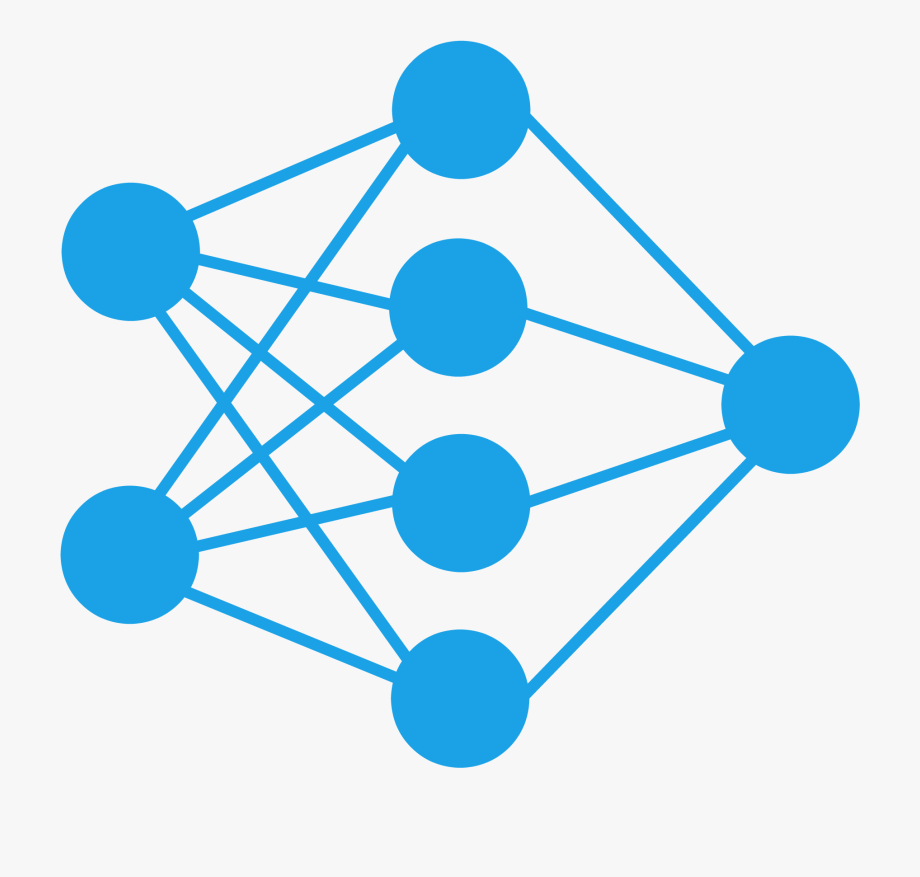
\includegraphics[scale=10]{./discussion/cover}
    \end{center}
\end{figure}

% Table des matières intro
{\LARGE
\begin{enumerate}[label=\textcolor{bleusection}{\arabic*}{.}, leftmargin=2cm]
  \item \nameref{discussion.1}
  \item \nameref{discussion.2}
  \item \nameref{discussion.3}
\end{enumerate}
}

\clearpage
\pagestyle{discussion}

\section{Avancées par rapport aux méthodes classiques de suivi}\label{discussion.1}
\subsection{Evaluation automatique de la diversité des récifs coralligènes}
\newpage
\subsection{Apports de la photogrammétrie par rapport à la télémétrie pour la cartographie des herbiers de Posidonie}
\newpage
\subsection{Caractérisation de la structure des récifs coralligènes}
\newpage
\subsection{Production de quadrats permanents}
\newpage


\section{Intégration aux réseaux de suivi des habitats marins}\label{discussion.2}
\subsection{RECOR: caractérisationo automatique des récifs coralligènes}
\newpage
\subsection{TEMPO: suivis temporels de la limite inférieure des herbiers}
\newpage

\subsection{Quadrats permanents pour le suivi de récifs coralligènes}
\subsubsection{Suivi d'impacts d'un chantier: cas du tombant des Spélugues à Monaco}
\newpage
\subsubsection{Suivi après restauration d'un récif: cas de Saint-Jean-Cap-Ferrat}
\newpage

\section{Perspectives de travail}\label{discussion.3}
\subsection{Couplage photogrammétrie et acoustique sous-marine: cartographie de l'activité biologique d'un récif coralligène}
\newpage
\subsection{Caractérisation du lien entre structure du coralligène et diversité ichtyologique}
\newpage
\subsection{Cartographie 3D automatique d'espèces du coralligène: couplage deep learning et photogrammétrie}